\newacronym{mimo}{MIMO}{\textit{Multiple Input Multiple Output}}
\newacronym{pid}{PID}{Proporcional Integral Derivativo}
\newacronym{mpc}{MPC}{Controle Preditivo Baseado em Modelo}
\chapter{Introdução}
\label{ch:introducao}

%Controle de processos é fundamental na industria.	[ok]
%Objetivo do controle.								[ok]
%Otimizar além de controlar.						[ok]
%Estratégias utilizando modelos matemáticos.		[ok]
%Porque não usar PID em alguns casos?				[ok - mais ou menos]
%Conceito do MPC.									[ok]
% TODO: (Brincalepe) Incluir histórico e maior detalhamento da importância do MPC atualmente
% TODO: (Brincalepe) Incluir citações
O controle de processos tem fundamental importância no desenvolvimento industrial,
sendo amplamente utilizado em praticamente todos os segmentos da indústria,
contribuindo de maneira significativa para a maior velocidade na estabilização de sinais,
aumento da qualidade de produtos, diminuição de riscos e redução de custos operacionais.
Seu objetivo, de forma simplificada, consiste em avaliar e corrigir desvios entre um
valor desejado e o real valor medido na saída da planta para uma dada variável do
processo (ou variáveis, como em casos de processos com múltiplas entradas e múltiplas
saídas, também conhecidos por sua sigla em inglês \acrshort{mimo} (\textit{\acrlong{mimo}})).
A aplicação correta de estratégias de controle acarreta numa operação eficiente da
planta, mantendo suas variáveis relevantes em condições próximas às desejadas.
A sintonia bem-feita do controle auxilia também na otimização do processo,
possibilitando que o sistema opere com menor variabilidade, maximizando a produção
e minimizando a utilização de recursos. No \cref{ch:otimizacao} abordaremos mais
sobre otimização.
Modelos matemáticos podem auxiliar a estratégia de controle uma vez que um modelo da
planta ou processo pode ser utilizado para estabelecer a relação existente entre as
variáveis manipuladas e variáveis controladas, assim podendo auxiliar na predição do
comportamento dinâmico do sistema analisado. A modelagem matemática pode ser feita
utilizando dados empíricos ou através da aplicação de relações físico-químicas.

% TODO: (Brincalepe) Incluir citações
A estratégia de controle predominante na indústria é o controle \acrshort{pid}
(\acrlong{pid}) que, além de levar em consideração o efeito proporcional (P) do erro
medido, também atua em desvios relativos aos efeitos integrais (I) e derivativos (D).
Seu elevado número de aplicações deve-se a uma grande variedade de vantagens como:
sua rápida implementação, facilidade de compreensão, disponibilidade em praticamente
todas as plataformas industriais de controle e principalmente pelo fato de não requerer
um modelo matemático do processo; porém apesar de poder ser aplicado com eficiência em
uma grande variedade de processos, o controle \acrshort{pid} aparece com menos frequência
em sistemas não-lineares, como em plantas de controle de pH, por exemplo. Em casos como
esse, outra técnica bastante utilizada na indústria (porém em proporções bem menores
que o \acrshort{pid}) pode ser utilizada: o controle \acrshort{mpc} (\acrlong{mpc},
do inglês \textit{Model Predictive Control}). Essa técnica consiste em predizer o
comportamento futuro de um sistema utilizando para isso um modelo do mesmo. Mais
detalhes sobre o \acrshort{mpc} serão apresentados no \cref{ch:mpc}.

% =====================================================================================================
% ============================================= Section ===============================================
% =====================================================================================================
\section{Objetivos}
\label{sec:objetivos}

Este trabalho propõe, como objetivo principal, desenvolver um controlador \acrshort{mpc}
aplicado a um sistema didático com restrições de atuação.

Além disso os seguintes objetivos específicos também serão realizados:
\begin{itemize}
    \item Estudo do algorítmo do controle \acrshort{mpc}
    \item Avaliação o desempenho do controlador \acrshort{mpc} desenvolvido em
        comparação com um controlador \acrshort{pid}
    \item Comparação entre a implementação em duas ou mais plataformas,
        como MATLAB\textsuperscript{\tiny\textregistered}\footnote{
            MATLAB\textsuperscript{\tiny\textregistered} é uma plataforma                           % Footnote
            de programação projetada especificamente para engenheiros e cientistas                  % Footnote
            onde é possível desenvolver algoritmos, realizar a análise de dados,                    % Footnote
            criar modelos, aplicações, dentre outras coisas.},                                      % Footnote
        Python\footnote{
            Python é uma linguagem de programação de alto nível,                                    % Footnote
            interpretada e orientada a objeto, muito utilizada atualmente para                      % Footnote
            aplicações nas áreas de ciência de dados, aprendizagem de máquina,                      % Footnote
            identificação de sistemas, etc.}                                                        % Footnote
        ou similares.
\end{itemize}

% =====================================================================================================
% ============================================= Section ===============================================
% =====================================================================================================
\section{Motivação e justificativas}
\label{sec:motivacao_e_justificativas}

% TODO: (Brincalepe) Incluir citações
% TODO: (Brincalepe) Paragrafo muito longo. Quebrar em pedaços
Segundo \citeonline{Parkinson2018} o processo de determinar o melhor \textit{design}
para uma aplicação ou processo é chamado de otimização. Normalmente engenheiros
costumam tentar implementar tais técnicas em seus processos visando aumentar a
eficiência diminuindo os gastos, por exemplo projetando o menor trocador de calor
que realize a transferência de calor desejada, uma ponte de menor custo para o local,
ou mesmo maximizar o rendimento de um processo químico, porém, assim como nesses
exemplos, as variáveis e limitantes do processo podem ser inúmeras, fazendo com que a
tarefa de otimização se torne difícil caso o engenheiro utilize apenas uma combinação
de experiência, conhecimento, opiniões, etc. Para esses casos, ferramentas
computacionais de otimização são essenciais.

Dá-se o nome de Otimização Dinâmica ao processo de otimização que é realizado
dinamicamente ao longo do processo e, segundo \citeonline{Borrelli2017}, esta se
tornou uma ferramenta padrão na tomada de decisões numa grande variedade de áreas.
O controle \acrshort{mpc} é um modo de implementação da otimização dinâmica e a execução
deste trabalho em torno dessa técnica se deve ao fato de que ao longo dos últimos 25 anos
ela evoluiu para dominar a indústria de processos, onde tem sido utilizada em milhares
de problemas \cite{Borrelli2017}, bem como no controle dos processos de fabricação de cimento,
torres de destilação, plantas de PVC \cite{Camacho2007}, e também ao seu crescimento em outras
indústrias, como por exemplo a descrita por \citeonline{Yakub2013} em seu estudo comparativo
mostrando a utilização do \acrshort{mpc} no controle do sistema dinâmico de um automóvel.

% =====================================================================================================
% ============================================= Section ===============================================
% =====================================================================================================
\section{Organização do trabalho}
\label{sec:organizacao_do_trabalho}

% TODO: (Brincalepe) Descrever este trecho como sendo um objetivo específico
Este trabalho, além de visar abordar uma implementação prática de um controle \acrshort{mpc}
também busca ser um ponto de partida teórico e experimental para estudantes de graduação ou
pós-graduação, de língua portuguesa, que possuam algum conhecimento sobre teoria de controle,
porém que ainda estejam iniciando suas pesquisas sobre otimização de processos e controle preditivo.

A \cref{fig:estrutura_do_trabalho} indica um possível fluxo de leitura desde trabalho, sendo importante
ressaltar que os \cref{ch:otimizacao,ch:controle_preditivo} servem de base para uma melhor
compreensão do \cref{ch:mpc} e, portanto, podem ser lidos sem respeitar a ordem numérica dos mesmos.

\begin{figure}[h]
    \caption{Diagrama do fluxo de leitura do trabalho}
    \begin{center}
		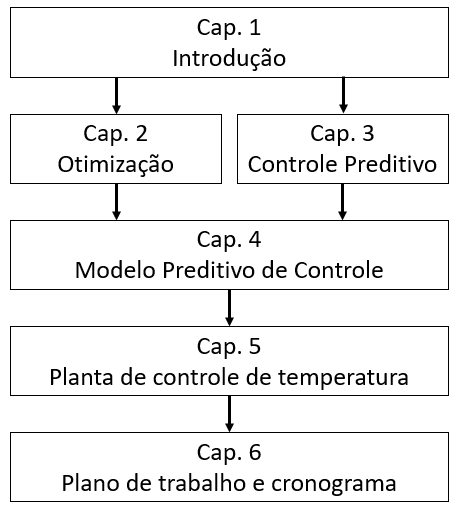
\includegraphics[width=0.4\textwidth]{./5_images/fig_estrutura_do_trabalho.png} 
		\label{fig:estrutura_do_trabalho}
    \end{center}
    \centering
    \makebox[\width]{Fonte: Autor}
\end{figure}